\usetikzlibrary{calc,arrows.meta,angles,quotes}
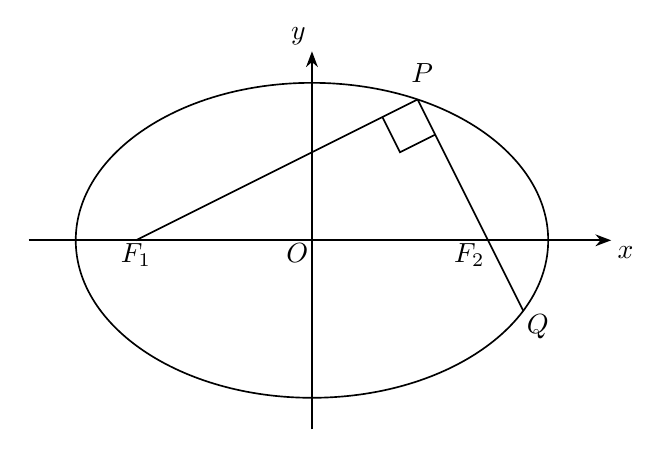
\begin{tikzpicture}[x=1cm,y=1cm,line width=.6pt,font=\normalsize,>=Stealth]
\coordinate (O) at (0,0);
\coordinate (F1) at (-2.2361,0);
\coordinate (F2) at (2.2361,0);
\coordinate (P) at (1.3416,1.7889);
\coordinate (Q) at (2.6833,-0.8944);
\draw[->] (-3.6,0)--(3.8,0) node[anchor=north west,inner sep=0pt,xshift=2pt,yshift=-2pt] {$x$};
\draw[->] (0,-2.4)--(0,2.4) node[anchor=south east,inner sep=0pt,xshift=-2pt,yshift=2pt] {$y$};
\draw (O) ellipse[x radius=3cm,y radius=2cm];
\draw (P)--(F1);
\draw (P)--(Q);
\pic[draw,line width=.6pt,angle radius=5mm] {right angle=F1--P--F2};
\node[below left,inner sep=1pt] at (O) {$O$};
\node[below,inner sep=1pt] at (F1) {$F_1$};
\node[below left,inner sep=1pt] at (F2) {$F_2$};
\node[inner sep=1pt] at (1.40,2.12) {$P$};
\node[below right,inner sep=1pt] at (Q) {$Q$};
\end{tikzpicture}
